%%%%%%%%%%%%%%%%%%%%% chapter.tex %%%%%%%%%%%%%%%%%%%%%%%%%%%%%%%%%
%
% sample chapter
%
% Use this file as a template for your own input.
%
%%%%%%%%%%%%%%%%%%%%%%%% Springer-Verlag %%%%%%%%%%%%%%%%%%%%%%%%%%
%\motto{Use the template \emph{chapter.tex} to style the various elements of your chapter content.}


\chapter{Network-aware Adaptive Listen Before Talk Co-existence Mechanism}
\label{intro-NALT} % Always give a unique label
% use \chaptermark{}
% to alter or adjust the chapter heading in the running head

%\abstract*{Each chapter should be preceded by an abstract (10--15 lines long) that summarizes the content. The abstract will appear \textit{online} at \url{www.SpringerLink.com} and be available with unrestricted access. This allows unregistered users to read the abstract as a teaser for the complete chapter. As a general rule the abstracts will not appear in the printed version of your book unless it is the style of your particular book or that of the series to which your book belongs.
%Please use the 'starred' version of the new Springer \texttt{abstract} command for typesetting the text of the online abstracts (cf. source file of this chapter template \texttt{abstract}) and include them with the source files of your manuscript. Use the plain \texttt{abstract} command if the abstract is also to appear in the printed version of the book.}
%TODO: Edit the abstract to be at least 1-2 lines shorter in the typeset document
\abstract{In the absence of coordination between radio access technologies, and with the goal of deploying unlicensed LTE without requiring changes to the Wi-Fi MAC layer, it falls to the LTE base stations to ensure fair coexistence.   The multiple access method used in 802.11 Wi-Fi is designed for fair sharing of the channel resources among devices with similar transmission and medium access profiles.  This can easily lead to Wi-Fi stations being barred from the channel if LAA-LTE is not designed to ensure fairness.  If no changes are to be made to Wi-Fi devices, then the greatest gains in fair coexistence are achieved when unlicensed LTE behaves in as Wi-Fi like a manner as possible, however, this may not allow LTE to make the best use of the channel.  In this chapter, a network-aware adaptive LBT mechanism (NALT) is proposed which passively monitors both channel conditions and usage activity to maximize its transmission opportunities while respecting fair sharing of the channel, in a way that is transparent to incumbent Wi-Fi devices.  Simulation results are presented showing the resulting proportional fair sharing which results from several independent NALT enable LAA-LTE networks sharing the channel with existing Wi-Fi stations.}

\section{Background and Theoretical Basis}
\label{background}
As discussed in Chapter \ref{overview-wifi}, \mbox{Wi-Fi} employs a fairly simple multiple access strategy which can be easily overwhelmed if competing devices are not also designed for fair coexistence. The \mbox{Wi-Fi} MAC protocol employs listen-before-talk (LBT) and is based on a probabilistic model of channel access which minimizes collisions through the use of random backoff to limit the probability that two stations will transmit at the same time after the channel has become idle \cite{80211}.  When a collision is inferred after a failed transmission, the set of possible backoff values grows exponentially to further reduce the probability of subsequent transmission failures.  While the ETSI LBT standard on which the recommended mechanism for \mbox{LAA-LTE} is based is also probabilistic, it employs a random backoff from a fixed set of possible backoff values \cite{3gpp}, which does not attempt to reduce the probability of collision on repeated failed transmission.  Thus, if a collision occurs, \mbox{Wi-Fi} will react by reducing its probability of gaining access to the channel, relative to a device modeled on the ETIS LBT mechanism.  Additionally, \mbox{LAA-LTE} used for supplemental downlink or carrier aggregation is expected to align subframes with the licensed band, and such subframes have a duration of $1$ms, which is significantly longer than the average channel occupancy time of a Wi-Fi station.  Combined, these two factors will lead to \mbox{LAA-LTE} stations winning the channel and then occupying the channel for significantly longer than an average competing \mbox{Wi-Fi} station would, even if the number of channel accesses were equal.  Since \mbox{Wi-Fi} stations may operate at any of several modulation and coding schemes, it is also difficult to provide throughput fairness unless \mbox{LAA-LTE} base stations monitor both however, using the principles developed for the $802.11$e Enhanced Distributed Channel Access (EDCA) function for service differentiation between traffic priorities, there are mechanism which can be leveraged to provide airtime fairness.  

In EDCA, \mbox{Wi-Fi} parameters such as contention window and inter-frame spacing are set up to provide quality of service differentiation among varying types of traffic by impacting the probabilities of gaining channel access \cite{80211}.  By changing these parameters, it is possible to impact the probability of channel access in a predictable way.  By constantly managing these parameters in response to network activity, it is possible to maintain long run proportionally fair sharing between the two types of competing networks.  

Specifically, the relationship between minimum contention window size for two traffic classes, and their relative proportion of channel access has been found to be

\begin{equation}\label{cw}
\frac{\theta_i}{\theta_j} \approx \frac{CW^j_{min}}{CW^i_{min}}
\end{equation}
where, $\sfrac{\theta_i}{\theta_j}$ is the proportion of channel access $i$ sees relative to class $j$, and $CW^x_{min}$ is the minimum contention window used by class $x$ \cite{chou}\cite{yoon}.  

To use Eq. \ref{cw} to balance airtime between \mbox{LAA-LTE} and \mbox{Wi-Fi}, it is necessary to treat all \mbox{Wi-Fi} stations and all LAA-LTE networks as single traffic classes and account for the duration of channel access for each class. Between the two traffic classes, this duration will generally be significantly longer for LAA-LTE than for Wi-Fi due to the synchronization between licensed and unlicensed transmissions. For example, if a \mbox{Wi-Fi} channel access takes half the time of a \mbox{LAA-LTE} channel access, in the case of a single \mbox{LAA-LTE} station competing with a single \mbox{Wi-Fi} station, the \mbox{Wi-Fi} station should receive twice as many transmission opportunities as the \mbox{LAA-LTE} station in order to achieve equal airtime.  If there were two \mbox{Wi-Fi} stations, in order for each to have equal airtime, the \mbox{LAA-LTE} station should receive one third as many transmission opportunities as the combined \mbox{Wi-Fi} stations, so that proportionally each of the three stations would receive equal airtime on average.  Adding some proportionality constants and solving Eq. \ref{cw} for the required $CW_{min}$ values to realize equal airtime,

\begin{equation}\label{cwlte}
CW^{LTE}_{min} = \rho\cdot{CW^{WiFi}_{min}}
\end{equation}
where $\rho$ is the ratio of \mbox{LAA-LTE} transmission time to average \mbox{Wi-Fi} transmission time.  This relation provides an approximation of the optimal $CW^{LTE}_{min}$ to provide airtime fairness, however, the \mbox{Wi-Fi} traffic class may be made up of stations which are using different transmission rates and $CW_{min}$ values.  

In order to estimate the $CW^{WiFi}_{min}$ to use in Eq. \ref{cwlte}, and adjust to changing network topologies, an estimate of the average current Wi-Fi contention window being used is required.  Such an estimate can be obtained from the number of collisions on the channel which are being inferred by the LAA-LTE base station from its own failed transmissions.  In a strictly \mbox{Wi-Fi} system, the probability of collision in a saturated network is given by, 

\begin{equation}\label{pcollision}
p = 1-(1-\sfrac{1}{CW_{avg}})^{n-1}
\end{equation}
where $CW_{avg}$ is the average contention window currently being employed in the network, and $n$ is the number of competing stations \cite{vu}.  Rearranging and solving for $CW_{avg}$ yields,
\begin{equation}\label{cwavg}
CW_{avg} = \frac{1}{1-e^{ \sfrac{ln(1-p)}{(n-1)} }}
\end{equation}
Eq. \ref{cwavg} provides the average contention window size for all stations.  In order to consider only the average contention window size for the \mbox{Wi-Fi} stations, and noting the optimal $CW^{LTE}_{min}$ to $CW^{WiFi}_{min}$ ratio, we can estimate $CW^{WiFi}_{min}$ as
\begin{equation}\label{cwwifi}
CW^{WiFi}_{avg} = CW_{avg}\left ( \frac{n_{WiFi} + n_{LTE}}{n_{WiFi} + \rho\cdot n_{LTE}} \right )
\end{equation}
then combining Eq. \ref{cwlte} through Eq. \ref{cwwifi},  we set 
\begin{equation}\label{cwlteopt}
CW^{LTE} = \rho \cdot{CW^{WiFi}_{avg}} = \frac{1}{1-e^{ \sfrac{ln(1-p)}{(n_{WiFi} + n_{LTE}-1)} }}\left ( \frac{n_{WiFi} + n_{LTE}}{n_{WiFi} + \rho\cdot n_{LTE}} \right )
\end{equation}

In order to use Eq. \ref{cwlteopt} in an implementable algorithm, the unknown probability of collision  $p$ and knowledge of the number of competing Wi-Fi stations and LAA-LTE networks is required.

\section{Proposed Mechanism}
\label{proposed}
NALT is defined as a simple distributed coordination function to be implemented by LAA-LTE base stations, allowing several LAA-LTE networks to effectively and independently fairly share the channel with each other and incumbent Wi-Fi stations. 

To gather the required information to utilize the relationships in the previous sections, the following assumptions are made:
\begin{itemize}
	\item NALT-enabled base stations are able to:
	\begin{itemize}
	\item Analyze traffic on the channel and determine the number of competing stations and their types, as is assumed in other coexistence mechanisms
	\item Determine average transmission durations either by decoding headers to determine the modulation and coding schemes employed, actually timing the transmissions, or some other suitable mechanism
	\end{itemize} 
	\item Successfully decoding a transmission implies that the transmission was successful (i.e. ignoring the hidden terminal problem) 
	\item Failed \mbox{LAA-LTE} transmissions can be reported to the base station on control channels in the licensed spectrum
\end{itemize}

In order to use Eq. \ref{cwlteopt} in an implementable algorithm, the unknown probability of collision  $p$ and knowledge of the number of competing Wi-Fi stations and LAA-LTE networks is required. Since these values cannot be known beforehand, the number of competitors is learned over time and the required probability of collision is estimated in each NALT-enabled LAA-LTE network as the ratio of observed \mbox{LAA-LTE} collisions to the number of \mbox{LAA-LTE} channel uses.  Noting that this is an empirical estimate of the true statistic, its reliability is inversely proportional to the number of samples and improves over time. The relationship in Eq. \ref{cwlteopt} is exploited to achieve fair airtime allocation by tuning the $CW_{min}$ values used by competing stations in each LAA-LTE network.  Since it is desired to avoid any changes to \mbox{Wi-Fi}, and fairer coexistence can be achieved by designing a more \mbox{``\mbox{Wi-Fi}-like"} MAC layer for \mbox{LAA-LTE}, i.e. the contention window used by \mbox{LAA-LTE} must increase as the number of collisions increases.  To facilitate fair airtime allocations across all competing devices, the contention window should follow Eq. \ref{cwlteopt}.  Based on the limitations of the estimates employed, and to ensure that the contention window stays within reasonable bounds, the maximum and minimum values for $CW^{LTE}$ are chosen to match the range of possible values for \mbox{Wi-Fi} \cite{80211}.  

Combining these requirements, and the preceding equations and assumptions, at each time instance an \mbox{LAA-LTE} station will estimate the average \mbox{Wi-Fi} contention window as follows:
\begin{align}
CW^{WiFi}_{avg} = CW^{WiFi}_{min}, \text{  if \{ \# of \mbox{Wi-Fi} Tx\}$> \rho\cdot$\{  \# of \mbox{LAA-LTE} Tx\}}\notag\\ 
\text{Otherwise, update according to Eq. \ref{cwwifi}.}
\end{align}
Thus, \mbox{LAA-LTE} will follow the same backoff procedure as \mbox{Wi-Fi}, and increase its contention window after a collision according to
\begin{align}
&CW^{LTE}=\;\;min\left[max\left(CW^{LTE}*2,\rho \cdot CW^{WiFi}_{avg}\right), CW^{LTE}_{MAX}\right]
\end{align}
and decreasing its contention window after a successful transmission according to 
\begin{align}
&CW^{LTE}=\;\;min\left[max\left(CW^{LTE}_{MIN},\rho \cdot CW^{WiFi}_{avg}\right), CW^{LTE}_{MAX}\right]
\end{align}

These equations, in addition to channel usage statistics gathering function, are implemented in each of the competing LAA-LTE base stations.  This mechanism requires no explicit coordination between the LAA-LTE base stations, nor any changes to Wi-Fi stations.

%TODO: Update with performance evaluation details, results, and edit from here down
\section{Performance Evaluation}\label{perf-eval}
To evaluate the performance of NALT, a high-level MATLAB simulation of a single \mbox{LAA-LTE} device contending with several \mbox{Wi-Fi} stations was developed and the proportion of channel accesses by each class of devices was tracked.  Simulating a small number of \mbox{LAA-LTE} devices is reasonable since it can be assumed that \mbox{LAA-LTE} user equipment will be coordinated via licensed band control channels, with scheduling done by the base station so that there is coordinated channel accesses for both uplink and downlink traffic.  Thus, each device in fact represents an independent network of LAA-LTE devices which are not required to contend with each other.


\subsection{System Model}
\label{sys-model}
For simplicity, we assume that both \mbox{LAA-LTE} and \mbox{Wi-Fi} stations use the same modulation and coding scheme and channel bandwidth, resulting in a data rate of $135$ Mbps.  Other than the adaptive contention window, the channel occupancy, and minimum time idle were modeled after ETSI LBE LBT and the proposed mechanisms for \mbox{LAA-LTE} \cite{3gpp}. The other pertinent simulation parameters are listed in Table \ref{params}.
\begin{table}
	\caption{NALT Simulation Parameters}
	\label{params}      
	\begin{tabular}{p{7cm}p{5cm}}
		\hline\noalign{\smallskip}
		Parameter & Value \\
		\noalign{\smallskip}\svhline\noalign{\smallskip}
		Number of competing \mbox{Wi-Fi} stations& $1 - 10$ \\ 
		Wi-Fi OFDM Symbol Duration (slot) & 9 $\mu$s    \\ 
		DCF Interframe Spacing $^1$ & 34 $\mu$s   \\ 
		Short Interframe Spacing $^1$ & 16 $\mu$s   \\ 
		\mbox{Wi-Fi} Frame Size & 1536 bytes  \\ 
		\mbox{Wi-Fi} Tx Duration $^2$(Frame Tx + SIFS +ACK) & 198 $\mu$s   \\ 
		Number of independent LTE Networks & 2 \\
		\mbox{LAA-LTE} Channel Occupancy Time  & 1000 $\mu$s \\ 	
		\noalign{\smallskip}\hline\noalign{\smallskip}
	\end{tabular}
	$^1$ Defined interframe spaces per 802.11n operating in the 5 GHz band \\
	$^2$ Based on header transmitted at lowest supported rate and remaining frame at specified bitrate	 
\end{table}

\subsection{Simulation Results}
\label{sim-results}

Since the coexistence mechanism is probabilistic, $1000$ trials were run for each considered network topology of between $1$ and $10$ \mbox{Wi-Fi} stations contending with a \mbox{LAA-LTE} station.  The average number of successful channel accesses was tracked across all trials and is related to airtime by the transmission duration of each class of devices.  The resulting proportion of airtime for each device when using NALT is shown in Fig. \ref{results}.
\begin{figure}[t] %TODO: new figures should be made to look better constructed
	\centering
	\subfloat[With LAA-LTE using NALT]{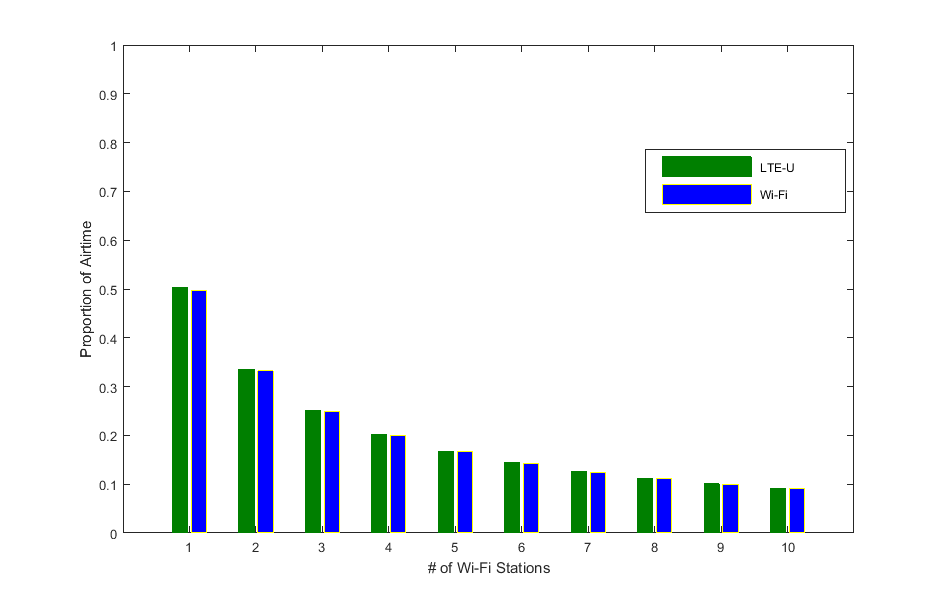
\includegraphics[width=3.5in]{figures/withadapt}%
		\label{results}}
	\hfil
	\subfloat[With LAA-LTE using ETSI LBE LBT]{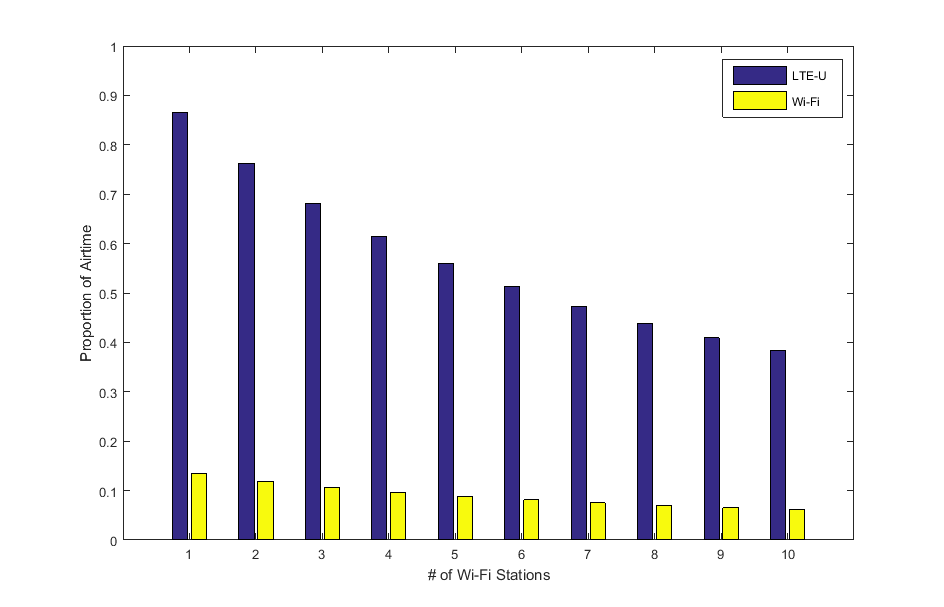
\includegraphics[width=3.5in]{figures/withoutadapt}%
		\label{fig_second_case}}
	\caption{Airtime allocations for each station type, normalized to number of stations, with and without NALT.}
	\label{compresults}
\end{figure}
For comparison, the simulation was run with the same parameters as in Table \ref{params}, but with a fixed contention window size of $16$, corresponding to the approximate midpoint of possible values under ETSI LBE LBT \cite{3gpp}. The resulting airtime allocations per device are shown in Fig. \ref{compresults}.

\section{Discussion and Future Work}
\label{future-work}
NALT requires no changes to \mbox{Wi-Fi} devices and in high-level simulations it shows promise in providing fair coexistence. As noted, several assumptions were made which affect the results.  It is reasonable that \mbox{LAA-LTE} would be able to analyze the channel and determine the number or competing \mbox{Wi-Fi} stations as well as their transmission bit rates, from the \mbox{Wi-Fi} preamble and MAC header.  The simulation assumed all \mbox{Wi-Fi} stations were using the same data rate, which should provide the same results as an average data rate, but the impact on individual \mbox{Wi-Fi} stations utilizing the channel access opportunities in a multi-rate environment was not explored.  Further, the impacts of hidden terminals, non-saturated stations, and lossy channels, were not explored, and may have interesting implications. The assumption that up/downlink traffic within a single \mbox{LAA-LTE} network would be centrally coordinated by the base station simplifies the problem. However, NALT does not consider the scenario where several uncoordinated \mbox{LAA-LTE} networks operate in the same frequency band.  Without coordination between unrelated \mbox{LAA-LTE} networks, contention between \mbox{LAA-LTE} user equipment, whether or not \mbox{Wi-Fi} devices are also present, will present a further challenge. Treating \mbox{LAA-LTE} devices in the same way as \mbox{Wi-Fi} devices when estimating contention parameters and average transmission rates and durations would potentially render the outcome invalid.  Further simulations of this scenario, and possibly adjustments to the algorithm to account for different classes of devices, is a necessary next step in the development of NALT.

%%%%%%%%%%%%%%%%%%%%%%%% referenc.tex %%%%%%%%%%%%%%%%%%%%%%%%%%%%%%
% sample references
% %
% Use this file as a template for your own input.
%
%%%%%%%%%%%%%%%%%%%%%%%% Springer-Verlag %%%%%%%%%%%%%%%%%%%%%%%%%%

\begin{thebibliography}{99.}%
	\bibitem{3gpp}{3GPP}, ``Feasibility study on licensed-assisted access to unlicensed spectrum,'' \emph{{TR 36.889 v13.0.0}}, July 2015.
	\bibitem{chou} C.~T. Chou, K.~G. Shin, and S.~Shankar, ``{Contention-based airtime usage control in multirate IEEE 802.11 wireless LANs},'' \emph{{IEEE/ACM Transactions on Networking}}, vol.~14, no.~6, pp. 1179--1192, December 2006.	
	\bibitem{80211}``{IEEE Standard for information technology--Telecommunications and information exchange between systems Local and metropolitan area networks--Specific requirements Part 11: Wireless LAN medium access control (MAC) and physical layer (PHY) specifications},'' \emph{{IEEE Std 802.11-2012 (Revision of IEEE Std 802.11-2007)}}, pp. 818--972, March 2012.	
	\bibitem{vu} H.~L. Vu and T.~Sakurai, ``{Collision probability in saturated IEEE 802.11 networks},'' in \emph{{Australian Telecommunication Networks \& Applications Conference}}, September 2006, pp. 1--5.
	\bibitem{yoon} {J. Yoon, S. Yun, et al}, ``{Maximizing differentiated throughput in IEEE 802.11e wireless LANs},'' in \emph{{ Proceedings of the 31st IEEE Conference on Local Computer Networks}}, vol.~14, no.~6, November 2006, pp. 411--417.
\end{thebibliography}


